%%%%%%%%%%%%%%%%%%%%%%%%%%%%%%%%%%%%%%%%%%%%%%%%%%%%%%%%%%%%%%%%%%%%%%%%%%%
%%  chapter1.tex  –  Глава 1: Обзор литературы и анализ пробелов
%%  v9 – Реструктурировано в соответствии с поэтапным охватом:
%%       НВ динамика → распределённость → эффективность → нестационарность.
%%       Покрыты все 12 пересечений 3 условий × 4 требований.
%%       Выявлены 7 пробелов. Связующие утверждения между разделами.
%%       Только заголовки \section добавлены в оглавление.
%%%%%%%%%%%%%%%%%%%%%%%%%%%%%%%%%%%%%%%%%%%%%%%%%%%%%%%%%%%%%%%%%%%%%%%%%%%

\chapter{Анализ гибридных систем обнаружения и предотвращения вторжений и теоретические основы повышения их робастности}
\label{ch:literature}

В настоящей главе представлен системный обзор гибридных систем
обнаружения и предотвращения вторжений (гибридная СОПВ) как объекта
исследования: даны определение и классификация гибридная СОПВ
(\S\ref{sec:hybrid_idps_object}), систематизированы предметные области
применения~--- защита сетевого трафика, систем БПЛА, финансово-технологической
инфраструктуры, медицинских данных, промышленного интернета вещей,
автономных транспортных средств и облачных сред,~--- проведена
таксономия моделей и алгоритмов, применяемых в гибридная СОПВ
(\S\ref{sec:idps_models_taxonomy}), и систематизированы проблемы и
уязвимости моделей в гибридная СОПВ (\S\ref{sec:idps_problems}).
Графовые нейронные сети рассматриваются в работе как одна из ветвей
семейства моделей, применяемых в гибридная СОПВ, наряду со
статистическими, классическими ML-, гибридными и теоретико-игровыми
подходами. После систематизации предметной области разделы
\ref{sec:gnn_vulnerability}--\ref{sec:certification} углубляются
в техническую базу разработки моделей М1--М7 по поэтапному охвату:
от динамики непрерывного времени на эволюционирующих графах, через
распределённое федеративное обучение с приватностью, к вычислительной
эффективности для крупномасштабных графов и, наконец, к
нестационарной адаптации с оценкой неопределённости. Каждый раздел
адресует одно или несколько пересечений трёх рабочих условий
(состязательная среда, распределённая динамика, нестационарность) и
четырёх сквозных требований (робастность, точность, эффективность,
приватность), выстраивая систематическое перечисление семи
исследовательских пробелов, мотивирующих модели и алгоритмы,
разработанные в Главе~\ref{ch:methods}.

Высокоуровневая интегрированная схема гибридной СОПВ,
систематически охватывающая источники данных, конвейер
нормализации, трёхканальное ядро детектирования (сигнатурное,
аномалийное, протокольный анализ) с AI-нативным интеллектуальным
слоем, единый менеджер решений и реагирования, перечень
защищаемых секторов с их характерными уязвимостями и обобщённые
свойства и выгоды развёртывания системы, приведена на
рис.~\ref{fig:hybrid_idps_executive}.

\begin{figure}[htbp]
\centering
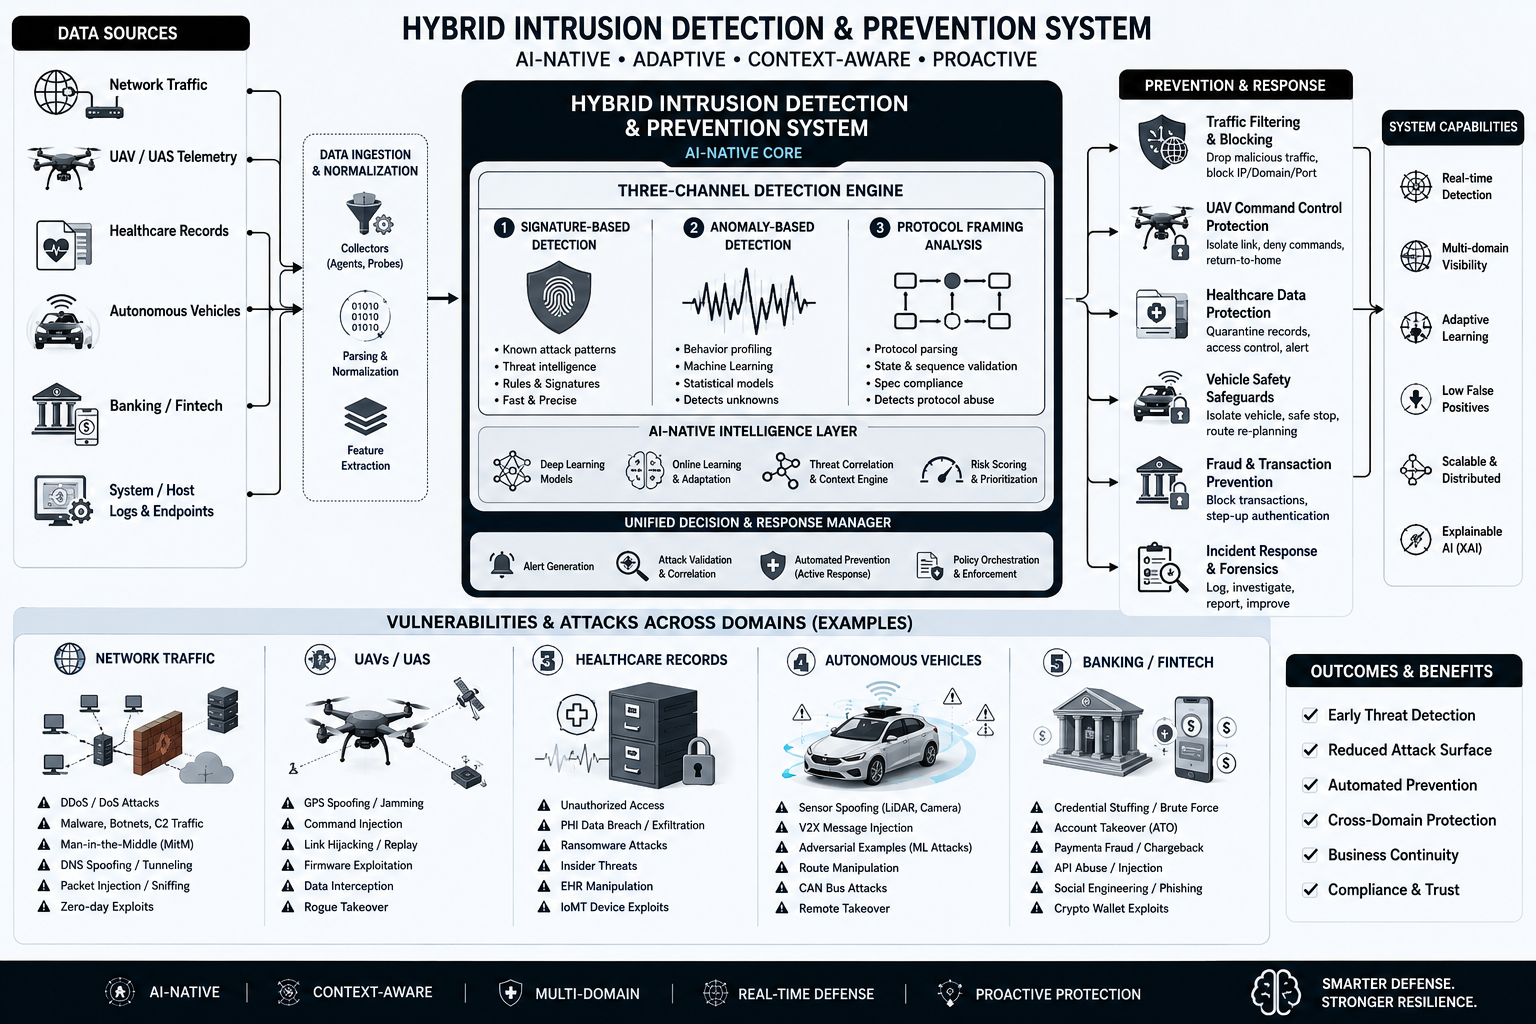
\includegraphics[width=\textwidth]{figures/fig_nidps_v1.png}
\caption{Интегрированная схема гибридной СОПВ:
AI-нативное, адаптивное, контекстно-зависимое, упреждающее
защитное решение. Слева~--- источники данных (сетевой трафик,
телеметрия БПЛА, медицинские записи, автономные транспортные
средства, банковский/финтех-трафик, системные журналы);
по центру~--- ядро системы с трёхканальным детектированием
(сигнатурное, аномалийное, протокольный анализ),
AI-нативным интеллектуальным слоем (глубокое обучение, онлайн-
обучение, корреляция угроз, оценка риска) и единым менеджером
решений и реагирования; справа~--- блок предотвращения и
реагирования (фильтрация трафика, защита команд БПЛА, защита
медицинских данных, активная безопасность транспортных средств,
предотвращение мошенничества, инцидент-форензика) и системные
возможности (обнаружение в реальном времени, многосекторная
видимость, адаптивное обучение, низкая доля ложных срабатываний,
масштабируемость, объяснимый ИИ). Нижняя панель приводит
характерные классы уязвимостей в каждом из пяти показательных
секторов.}
\label{fig:hybrid_idps_executive}
\end{figure}


%%=====================================================================
\section{гибридная СОПВ как объект исследования: определение, классификация и предметные области применения}
\label{sec:hybrid_idps_object}
%%=====================================================================

\emph{Гибридной системой обнаружения и предотвращения вторжений}
(гибридная СОПВ) в настоящей диссертации называется \emph{ИИ/МО-нативный}
программно-аппаратный комплекс защиты информационных систем,
объединяющий в едином защитном контуре три канонических типа
детектирования информационной безопасности~--- \emph{сигнатурный}
(детерминированное сопоставление с базой известных шаблонов атак),
\emph{аномалийный} (статистическое или обучаемое отклонение от
нормального профиля поведения) и \emph{протокольный анализ}
(контекстно-зависимый разбор корректности сетевых, прикладных и
индустриальных протоколов с учётом их состояний),~--- усиленных
обучаемыми моделями на каждом из трёх каналов и дополненных
средствами автоматического реагирования и интерфейсами интеграции с
внешними системами регистрации событий и реагирования (SIEM/SOAR).
В отличие от \emph{конвенциональных} IDPS-продуктов отрасли (Snort,
Suricata, Zeek, Cisco~IPS, Palo Alto~Threat~Prevention) гибридная СОПВ
в смысле настоящей диссертации систематически отличается от
классических IDS \emph{четырьмя} свойствами: \emph{(i)}~\emph{гибридностью} обнаружения~--- решение о
наличии вторжения принимается комбинацией нескольких независимых
детекторов, статистических признаков и обучаемых моделей с разной
степенью объяснимости; \emph{(ii)}~\emph{адаптируемостью} к
предметной области~--- одна и та же базовая архитектура может быть
инстанцирована в защиту сетевого трафика, систем БПЛА,
банковско-финансовой инфраструктуры, медицинских данных,
промышленного интернета вещей и иных областей за счёт смены
формального представления входных данных; \emph{(iii)}~\emph{обратной
связью реагирования}~--- наряду с обнаружением гибридная СОПВ
способен инициировать активное противодействие угрозе через изменение
правил межсетевого экрана, изоляцию узлов, переключение сенсорных
конвейеров или передачу события в SOAR-оркестратор;
\emph{(iv)}~\emph{ИИ-нативностью}~--- обучаемые модели~М1--М7,
разработанные в Главе~\ref{ch:methods}, интегрированы во все три
канала детектирования (сигнатурный, аномалийный, протокольный) для
систематического преодоления трёх неэффективностей конвенциональных
IDPS (см.~Введение): задержки сигнатурных баз в 30--90~дней,
частоты ложных срабатываний $10^{-2}$--$10^{-1}$ на нормальный
поток и квадратичной стоимости протокольного анализа по числу
протоколов и состояний.

\subsection{Классификация гибридная СОПВ}
\label{subsec:idps_classification}

Известные в литературе системы IDPS поддаются классификации по пяти
ортогональным осям: по применяемому методу обнаружения, по охвату
наблюдаемой среды, по сетевой топологии развёртывания, по
характеру реагирования и по уровню стека протоколов. Структура
классификации приведена на рис.~\ref{fig:orga_classes_idps}.

\begin{figure}[htbp]
\centering
\resizebox{\textwidth}{!}{%
\begin{tikzpicture}[
  font=\footnotesize,
  level 1/.style={sibling distance=33mm, level distance=11mm},
  level 2/.style={sibling distance=11mm, level distance=10mm},
  root/.style={draw,rounded corners=3pt,fill=blue!18,
    minimum width=3.5cm,minimum height=8mm,align=center,
    font=\small\bfseries,thick},
  cat/.style={draw,rounded corners=2pt,fill=blue!8,
    minimum width=2.4cm,minimum height=7mm,align=center,
    font=\scriptsize\bfseries,thick},
  leaf/.style={draw,rounded corners=2pt,fill=gray!10,
    minimum width=1.0cm,minimum height=6mm,align=center,
    font=\scriptsize,inner sep=2pt},
  edge from parent/.style={draw,gray!70!black,thick}]
\node[root] {гибридная СОПВ}
  child {node[cat] {По методу}
    child {node[leaf] {Сигн.}}
    child {node[leaf] {Аном.}}
    child {node[leaf] {Прот.}}
    child {node[leaf] {Гибр.}}}
  child {node[cat] {По охвату}
    child {node[leaf] {HIDS}}
    child {node[leaf] {NIDS}}
    child {node[leaf] {DIDS}}}
  child {node[cat] {По топологии}
    child {node[leaf] {Центр.}}
    child {node[leaf] {Распр.}}
    child {node[leaf] {Федер.}}}
  child {node[cat] {По реакции}
    child {node[leaf] {Пасс.}}
    child {node[leaf] {Акт.}}
    child {node[leaf] {IPS}}}
  child {node[cat] {По уровню}
    child {node[leaf] {App}}
    child {node[leaf] {Net}}
    child {node[leaf] {Phy}}};
\end{tikzpicture}%
}
\caption{Иерархическая классификация гибридная СОПВ по пяти
ортогональным осям. По методу обнаружения~--- сигнатурные
(детерминированный поиск по базе известных шаблонов), аномалийные
(статистическое или обучаемое отклонение от нормального профиля),
протокольные (контекстно-зависимый анализ корректности сетевых,
прикладных и индустриальных протоколов и их состояний) и гибридные
(комбинация трёх предыдущих, усиленная обучаемыми моделями~М1--М7).
По охвату~--- хостовые (HIDS), сетевые (NIDS) и распределённые (DIDS).
По топологии развёртывания~--- централизованные, распределённые,
федеративные. По характеру реагирования~--- пассивные (только
оповещение), активные (вмешательство в поток), IPS (полная
блокировка). По уровню стека~--- прикладной, сетевой и физический.}
\label{fig:orga_classes_idps}
\end{figure}

В рамках настоящей диссертации центральное внимание уделяется
гибридным системам распределённой топологии, действующим на сетевом
и прикладном уровнях, с активным реагированием.

\subsection{Предметные области применения гибридная СОПВ}
\label{subsec:idps_sectors}

гибридная СОПВ как универсальный защитный контур применим в широком
спектре предметных областей. На рис.~\ref{fig:orga_apps_idps}
приведена систематизация семи практически значимых секторов, для
каждого из которых ниже даны краткие постановочные сведения о
поверхности атак и специфике интеграции защитных моделей. Полные
системные реализации для двух показательных секторов~--- защиты
сетевого трафика и защиты беспилотных летательных аппаратов~---
изложены в Главах~\ref{ch:platform} и~\ref{ch:uav} соответственно.

\begin{figure}[htbp]
\centering
\resizebox{\textwidth}{!}{%
\begin{tikzpicture}[
  font=\footnotesize,
  level 1/.style={sibling distance=22mm, level distance=13mm},
  root/.style={draw,rounded corners=3pt,fill=orange!20,
    minimum width=4.6cm,minimum height=8mm,align=center,
    font=\small\bfseries,thick},
  sec/.style={draw,rounded corners=2pt,fill=orange!10,
    minimum width=1.8cm,minimum height=11mm,align=center,
    font=\scriptsize\bfseries,thick,inner sep=2pt},
  edge from parent/.style={draw,gray!70!black,thick}]
\node[root] {гибридная СОПВ Applications}
  child {node[sec,fill=orange!25] {(а)\\NIDS\\\scriptsize Глава~\ref{ch:platform}}}
  child {node[sec,fill=orange!25] {(б)\\UAV\\\scriptsize Глава~\ref{ch:uav}}}
  child {node[sec] {(в)\\Финтех}}
  child {node[sec] {(г)\\Медицина}}
  child {node[sec] {(д)\\IIoT/\\SCADA}}
  child {node[sec] {(е)\\Автоном.\\ТС}}
  child {node[sec] {(ж)\\Cloud/\\SaaS}};
\end{tikzpicture}%
}
\caption{Предметные области применения гибридная СОПВ. Сектора~(а) и~(б)
рассматриваются в работе как показательные применения и
изложены подробно в Главах~\ref{ch:platform} (анализ сетевого
трафика) и~\ref{ch:uav} (защита БПЛА). Сектора~(в)--(ж) приведены
обзорно с указанием поверхности атак и режима интеграции защитных
моделей.}
\label{fig:orga_apps_idps}
\end{figure}

\paragraph{(а) Защита сетевого трафика (NIDS)}\label{subsubsec:sector_nids}

Защита сетевого трафика исторически является первой и наиболее
изученной областью применения IDPS. Объектом наблюдения служит
последовательность сетевых пакетов и потоков, агрегированных в
многомерные признаковые векторы (для бенчмарков CIC-IoT-2023,
CSE-CICIDS-2018, UNSW-NB15~--- 46--83-мерные векторы). Поверхность
атак включает сканирование портов, эксплуатацию уязвимостей служб,
отказ в обслуживании (DoS/DDoS), горизонтальное распространение,
управляющие каналы (C2), эксфильтрацию данных и постквантовые
протокольные переходы. гибридная СОПВ интегрируется в стек защиты как
дополнение к классическим сигнатурным движкам (Snort, Suricata) и
получает на вход агрегированные признаки потоков, событийные графы
взаимодействия узлов и потоки SIEM-оповещений. Полное системное
описание данного сектора~--- Глава~\ref{ch:platform}.

\paragraph{(б) Защита беспилотных летательных аппаратов (UAV)}\label{subsubsec:sector_uav}

Защита БПЛА является показательным расширением гибридная СОПВ за
пределы традиционного сетевого периметра. Объектом наблюдения служит
гетерогенный поток телеметрии бортовых сенсоров (ИНС/ГНСС, ЛиДАР,
оптический поток, состояние двигателей и полезной нагрузки) в
сочетании с командно-телеметрическим каналом борт--дронопорт--облако.
Поверхность атак включает спуфинг и подавление сигналов ГНСС,
радиоэлектронную борьбу (РЭБ), состязательные атаки на бортовые
нейросетевые модули зрительного восприятия, отравление политик
автопилота, перехват командного канала, а также кинетические и
биологические угрозы (столкновения, атаки хищных птиц). гибридная СОПВ
адаптируется к данной среде через переход от граф-представления
сетевого трафика к граф-представлению операционной обстановки БПЛА с
сохранением неизменности математического аппарата М1--М7. Полное
системное описание~--- Глава~\ref{ch:uav}.

\paragraph{(в) Защита банковской и финансово-технологической инфраструктуры}\label{subsubsec:sector_fintech}

Объектом защиты выступают графы транзакций между счетами,
платёжными картами, торговыми точками и интерфейсами быстрых
платежей. Поверхность атак включает кардинг, отмывание денежных
средств, рейдовые транзакционные атаки на детекторы мошенничества
(MonTi-атака~\cite{MonTi2025} утраивает ошибку классификации
CARE-GNN/PC-GNN/GAGA с 25{,}7\% до 68{,}6\%), спуфинг учётных
данных, фишинг и атаки на системы оценки кредитоспособности.
гибридная СОПВ в финтех-секторе действует в условиях
\emph{сильного дисбаланса классов} (доля мошеннических транзакций
$<\!1\%$) и \emph{регуляторных ограничений} на использование
персональных данных, что требует одновременной византийской
устойчивости византийско-устойчивого федеративного обучения между банками
и сертифицированной устойчивости детектора к состязательным
переоформлениям транзакционных подграфов~--- методы для обоих
требований разрабатываются в Главе~\ref{ch:methods}.

\paragraph{(г) Защита медицинских информационных систем}\label{subsubsec:sector_medical}

Объектом защиты служат графы электронных медицинских карт, графы
взаимодействия пациент--врач--лаборатория, а также графы
молекулярных представлений в задачах фармакологии. Поверхность атак
включает атаки на чувствительность связей в графовых изоморфных
сетях (падение AUC до 25\% на бенчмарках MoleculeNet, при котором
токсичные соединения классифицируются как
безопасные~\cite{EdgeSensitivity2025}), атаки на конфиденциальность
обучающих данных (модельная инверсия, атаки на принадлежность к
обучающей выборке) и отравление графов клинических исследований.
гибридная СОПВ в медицинском секторе должен обеспечивать строгое
$(\varepsilon,\delta)$-дифференциально-приватное обучение и калиброванную оценку эпистемической неопределённости для отделения недостоверных предсказаний от достоверных.

\paragraph{(д) Защита промышленного интернета вещей и АСУ ТП (IIoT/SCADA)}\label{subsubsec:sector_iiot}

Промышленный интернет вещей и системы автоматизированного управления
технологическими процессами (АСУ ТП) технически отличаются от
традиционных NIDS-сред тремя обстоятельствами, что делает
IIoT/SCADA отдельной предметной областью применения гибридная СОПВ, а
не частным случаем сектора~(а):
\emph{(i)}~стек протоколов передачи данных опирается на
специализированные индустриальные протоколы (\texttt{Modbus},
\texttt{DNP3}, \texttt{IEC~61850}, \texttt{OPC-UA}, \texttt{S7}) с
семантикой управляющих регистров, отсутствующей в стеке TCP/IP;
\emph{(ii)}~операционные ограничения требуют детерминированной
задержки реакции в пределах десятков миллисекунд, что исключает
применение тяжёлых неэффективных моделей;
\emph{(iii)}~модель угроз включает специфические для индустрии классы~---
манипуляцию состоянием программируемых логических контроллеров
(ПЛК), повтор сигналов с датчиков и атаки на временные метки
синхронизации. Отравление обучающих данных федеративных детекторов
вторжений в IIoT-сетях зафиксировано как причина коллапса точности
с 94{,}2\% до 30{,}0\% при не-i.i.d.\ условиях
обучения~\cite{FerragPoisoning2023}. гибридная СОПВ в IIoT-секторе
реализуется на основе моделей, разработанных в Главе~\ref{ch:methods}.

\paragraph{(е) Защита автономных транспортных средств}\label{subsubsec:sector_av}

Объектом защиты в автономных транспортных средствах является граф
слияния сенсоров (камера, ЛиДАР, радар, ИНС), граф взаимодействия
с другими участниками движения через каналы V2X/V2I и граф
программных компонентов автопилота. Поверхность атак включает
состязательные физические заплатки на дорожные знаки, спуфинг
ГНСС, инжекцию ложных V2X-сообщений и отравление траекторного
планировщика. Сектор отличается от сектора~(б) тем, что
действующие лица находятся в наземной среде с другими
законодательными ограничениями и иной топологией информационного
обмена. гибридная СОПВ в данном секторе использует калиброванной оценки эпистемической неопределённости как
триггера перехода в безопасный режим.

\paragraph{(ж) Защита облачных и SaaS-инфраструктур}\label{subsubsec:sector_cloud}

Защита облачных и SaaS-инфраструктур также технически отличается от
традиционных NIDS-сред и не сводится к сектору~(а) по следующим
причинам:
\emph{(i)}~основным наблюдаемым потоком является не поток
сетевых пакетов, а поток вызовов прикладных программных интерфейсов
(API) между микросервисами (так называемый east--west-трафик),
наблюдаемый через инфраструктуру сервисного меша
(\texttt{Istio}, \texttt{Linkerd});
\emph{(ii)}~требуется обязательная многоарендная (\emph{multi-tenant})
изоляция между арендаторами облака, отсутствующая в традиционных
сетевых средах;
\emph{(iii)}~модель угроз включает специфические для облака классы~---
побег из контейнера, злоупотребление учётными записями систем
управления идентификацией и доступом (IAM), атаки на цепочку
поставок программного обеспечения и подмену образов контейнеров.
Атака PROVNINJA~\cite{PROVNINJA2023}, снижающая обнаружение
ГНС-систем на основе провенанса до 59\%, документально подтверждает
необходимость защиты данного сектора. гибридная СОПВ в облачном
секторе реализуется через модели, разработанные в Главе~\ref{ch:methods}.


%%=====================================================================
\section{Модели и алгоритмы, применяемые в гибридная СОПВ: систематизация подходов}
\label{sec:idps_models_taxonomy}
%%=====================================================================

Совокупность моделей и алгоритмов, применяемых в гибридная СОПВ,
систематизирована на рис.~\ref{fig:orga_models_idps} по пяти
семействам: статистические модели, классические алгоритмы
машинного обучения, модели глубокого обучения, гибридные подходы и
теоретико-игровые алгоритмы. Графовые нейронные сети (ГНС)
рассматриваются как один из листов ветви глубокого обучения~---
наряду с свёрточными, рекуррентными, трансформерными моделями и
моделями пространства состояний~--- а не как центральная парадигма.

\begin{figure}[htbp]
\centering
\resizebox{\textwidth}{!}{%
\begin{tikzpicture}[
  font=\footnotesize,
  level 1/.style={sibling distance=34mm, level distance=11mm},
  level 2/.style={sibling distance=10mm, level distance=10mm},
  root/.style={draw,rounded corners=3pt,fill=green!18,
    minimum width=4.2cm,minimum height=8mm,align=center,
    font=\small\bfseries,thick},
  fam/.style={draw,rounded corners=2pt,fill=green!8,
    minimum width=2.4cm,minimum height=8mm,align=center,
    font=\scriptsize\bfseries,thick},
  leaf/.style={draw,rounded corners=2pt,fill=gray!10,
    minimum width=0.9cm,minimum height=6mm,align=center,
    font=\scriptsize,inner sep=2pt},
  hi/.style={draw=red!70!black,fill=red!12,thick},
  edge from parent/.style={draw,gray!70!black,thick}]
\node[root] {Модели и алгоритмы в гибридная СОПВ}
  child {node[fam] {Статист.}
    child {node[leaf] {Bayes}}
    child {node[leaf] {Markov}}
    child {node[leaf] {HMM}}}
  child {node[fam] {Класс.\ ML}
    child {node[leaf] {SVM}}
    child {node[leaf] {RF}}
    child {node[leaf] {kNN}}}
  child {node[fam] {Глубокое обуч.}
    child {node[leaf] {CNN}}
    child {node[leaf] {RNN}}
    child {node[leaf,hi] {GNN}}
    child {node[leaf] {SSM}}}
  child {node[fam] {Гибридные}
    child {node[leaf] {Stack}}
    child {node[leaf] {Ens.}}}
  child {node[fam] {Теор.-игр.}
    child {node[leaf] {MAB}}
    child {node[leaf] {Stack.}}};
\end{tikzpicture}%
}
\caption{Систематизация моделей и алгоритмов, применяемых в
гибридная СОПВ. Графовые нейронные сети (выделены красной рамкой)
являются одним из листов ветви глубокого обучения наряду с
свёрточными (CNN), рекуррентными (RNN), моделями пространства
состояний (SSM) и стохастическими дифференциальными уравнениями
(SDE), а не центральной парадигмой. Разработанные в Главе~2 модели
М1--М7 заимствуют конструкции из нескольких ветвей одновременно
(см.\ табл.~\ref{tab:models_to_methods}).}
\label{fig:orga_models_idps}
\end{figure}

Каждое семейство моделей имеет характерные сильные и слабые стороны,
определяющие область его применимости в задачах гибридная СОПВ.
Статистические модели и классические алгоритмы машинного обучения
эффективны на низкоразмерных табличных признаках и предоставляют
интерпретируемые границы принятия решений, однако не способны
автоматически извлекать абстрактные представления из необработанных
сенсорных потоков и не масштабируются до миллионных размеров
графов. Модели глубокого обучения~--- CNN, RNN, трансформеры, GNN,
SSM, SDE~--- обеспечивают сквозное обучение признаков, однако
страдают от чувствительности к состязательным возмущениям и
требуют значительных вычислительных ресурсов на этапе вывода.
Гибридные подходы (стекинг, ансамбли, конвейерные архитектуры)
комбинируют сильные стороны разных семейств. Теоретико-игровые
алгоритмы (многоруких бандитов, равновесия Штакельберга, обучение с
подкреплением) применяются для онлайн-выбора стратегий реагирования
при адаптивном противнике. Соответствие разработанных в работе
моделей~М1--М7 ветвям приведённой таксономии задаёт область
ответственности каждой модели и допускает прямое отображение на
направление~п.\,4 паспорта специальности~2.3.1.

%%---------------------------------------------------------------------
\subsection{Современные коммерческие ИИ-усиленные IDPS-продукты}
\label{subsec:commercial_ai_idps}
%%---------------------------------------------------------------------

С 2023--2025~гг. ведущие производители средств защиты информации
ввели в эксплуатацию класс \emph{ИИ-усиленных} (AI-augmented)
коммерческих платформ обнаружения и реагирования, надстраиваемых
поверх классических сигнатурных и поведенческих движков.
Систематический обзор этого класса позволяет позиционировать
разработанный в работе каркас RobustIDPS.ai по отношению к
действующему промышленному уровню.

\begin{enumerate}[leftmargin=2em, itemsep=0.2em]

\item \textbf{CrowdStrike Falcon с модулем Charlotte~AI}~---
EDR/XDR-платформа с интегрированным LLM-ассистентом для
ускоренного анализа предупреждений и автоматического построения
сценариев реагирования; ядро обнаружения опирается на
поведенческие индикаторы атаки (IOA) и графы процессов.
Декларируемое преимущество~--- сокращение времени реагирования
SOC-аналитика; ограничения~--- закрытый кодекс правил,
отсутствие формальных сертификатов робастности к состязательным
воздействиям и зависимость от облачного бэкенда CrowdStrike.

\item \textbf{SentinelOne Singularity с Purple~AI}~---
автономная XDR-платформа с агентным ИИ для расследования
инцидентов на естественном языке; реализует поведенческое
обнаружение на агентном уровне и автоматизированный rollback при
ransomware. Ограничения, релевантные настоящей работе:
отсутствие формальной модели приватности при федеративном
обучении на данных нескольких заказчиков и отсутствие
сертифицированной устойчивости к атакам отравления обучающих
данных.

\item \textbf{Microsoft Security Copilot}~--- надстройка над
семейством Defender~XDR / Sentinel SIEM на основе GPT-семейства
LLM; ориентирована на расширение возможностей оператора SOC
(резюмирование инцидентов, генерация KQL-запросов, построение
плана реагирования). Принципиальное ограничение~--- решения LLM
не сопровождаются количественной оценкой неопределённости и не
имеют формальных гарантий робастности при состязательных
подсказках (prompt-injection).

\item \textbf{Google Cloud Threat Intelligence (Mandiant +
Gemini)}~--- интегрирует индикаторы компрометации Mandiant с
LLM-ассистентом Gemini для атрибуции и приоритизации угроз;
сильная сторона~--- агрегированные потоки разведданных, слабая
сторона~--- закрытость моделей и отсутствие гарантий для
on-premise развёртываний.

\item \textbf{Cisco AI Endpoint Analytics / Hypershield}~---
направлен на сегментацию сети и обнаружение аномалий на уровне
рабочих станций средствами обучаемых моделей идентификации
устройств; представляет собой коммерческий аналог моделей
обучения признаков для NIDPS, рассмотренных в подразделе~1.6.

\item \textbf{IBM QRadar SIEM AI Assistant} и \textbf{Palo~Alto
Networks Cortex~XSIAM}~--- ИИ-усиленные SIEM/SOAR-платформы;
обеспечивают автоматизированную корреляцию событий и
рекомендательные системы для аналитика, не предоставляя при этом
сертифицированных гарантий устойчивости к состязательным
воздействиям и не реализуя федеративного обучения между
организациями.

\end{enumerate}

\noindent Систематический разбор перечисленных продуктов
показывает, что \emph{все} они являются конвейерными надстройками
LLM/EDR над классическими движками, в которых отсутствуют:
(i)~единая математическая модель гибридная СОПВ как объекта
исследования с формальными гарантиями робастности,
(ii)~сертифицированная устойчивость к состязательным атакам с
доказательством по Липшицу или рандомизированным сглаживанием,
(iii)~приватные алгоритмы распределённого обучения с
дифференциальной приватностью и византийско-устойчивой
агрегацией, (iv)~калиброванная декомпозиция эпистемической и
алеаторной неопределённости. Эти четыре аспекта составляют
содержательное отличие разработанных в настоящей работе моделей
М1--М7 и платформы RobustIDPS.ai от рассмотренных коммерческих
ИИ-усиленных IDPS-продуктов; количественное сопоставление
проводится в Главе~\ref{ch:platform} (раздел
<<Сравнение с коммерческими и открытыми платформами>>).


%%=====================================================================
\section{Проблемы и уязвимости моделей в гибридная СОПВ}
\label{sec:idps_problems}
%%=====================================================================

Множество проблем, рассматриваемых в работе как мотивирующих
разработку моделей и алгоритмов М1--М7, систематизировано на
рис.~\ref{fig:orga_problems_idps}. Проблемы разнесены по пяти
кросс-секущим осям: робастность к состязательным воздействиям,
точность в условиях нестационарности и дисбаланса классов,
эффективность вывода в условиях ограниченных бюджетов,
дифференциальная приватность в распределённых средах и нестационарная
адаптация при дрейфе распределения.

\begin{figure}[htbp]
\centering
\resizebox{\textwidth}{!}{%
\begin{tikzpicture}[
  font=\footnotesize,
  level 1/.style={sibling distance=36mm, level distance=11mm},
  level 2/.style={sibling distance=12mm, level distance=11mm},
  root/.style={draw,rounded corners=3pt,fill=red!18,
    minimum width=4.6cm,minimum height=8mm,align=center,
    font=\small\bfseries,thick},
  ax/.style={draw,rounded corners=2pt,fill=red!8,
    minimum width=2.4cm,minimum height=8mm,align=center,
    font=\scriptsize\bfseries,thick},
  leaf/.style={draw,rounded corners=2pt,fill=gray!10,
    minimum width=1.2cm,minimum height=7mm,align=center,
    font=\scriptsize,inner sep=2pt},
  edge from parent/.style={draw,gray!70!black,thick}]
\node[root] {Проблемы и уязвимости гибридная СОПВ}
  child {node[ax] {Робаст.}
    child {node[leaf] {Adv.\\примеры}}
    child {node[leaf] {Отравл.}}
    child {node[leaf] {Бэкдор}}}
  child {node[ax] {Точность}
    child {node[leaf] {Дрейф}}
    child {node[leaf] {Дисба\-ланс}}
    child {node[leaf] {Few-shot}}}
  child {node[ax] {Эффект.}
    child {node[leaf] {Задерж.}}
    child {node[leaf] {Память}}
    child {node[leaf] {Пропуск}}}
  child {node[ax] {Приват.}
    child {node[leaf] {Инверс.}}
    child {node[leaf] {Memb.\\inf.}}
    child {node[leaf] {Утечки}}}
  child {node[ax] {Нестац.}
    child {node[leaf] {Дрейф\\распр.}}
    child {node[leaf] {Online}}};
\end{tikzpicture}%
}
\caption{Систематизация проблем и уязвимостей, рассматриваемых в
качестве мотивации для разработки моделей М1--М7. Каждая из пяти
осей покрывается одной или несколькими разработанными моделями
(прямое отображение приведено в табл.~\ref{tab:models_to_methods}
после изложения существующих ограничений).}
\label{fig:orga_problems_idps}
\end{figure}

Соответствие осей рис.~\ref{fig:orga_problems_idps} разработанным
моделям задаёт прямое отображение направлений исследований паспорта
специальности~2.3.1 (п.\,4 и п.\,5) на содержательные результаты
диссертации: ось~\emph{робастность} покрывается моделями М1, М4 и
М5--М6; ось~\emph{точность}~--- М1, М3 и М5--М6; ось~\emph{эффективность}~---
М4 и М7; ось~\emph{приватность}~--- М2; ось~\emph{нестационарность}~--- М1,
М3 и М6.


%%=====================================================================
\section{Графовые нейронные сети: архитектура, уязвимость и проблема двойного входа}
\label{sec:gnn_vulnerability}
%%=====================================================================

\subsection{Архитектура передачи сообщений и агрегация окрестностей}

Графовые нейронные сети~\cite{Kipf2017,Velickovic2018,Hamilton2017} расширяют глубокое обучение на неевклидовы реляционные данные путём итеративной агрегации информации от соседей узла. Каноническая формулировка передачи сообщений обновляет представление узла $v$ на слое $k+1$ как
\begin{equation}
\bh_v^{(k+1)}
= \phi\!\Bigl(\bh_v^{(k)},\;
  \bigoplus_{u\in\calN(v)}
    \psi\!\bigl(\bh_u^{(k)},\, \mathbf{e}_{uv}\bigr)\Bigr),
\label{eq:ch1_mp}
\end{equation}
где $\phi$ и $\psi$ --- обучаемые функции, $\bigoplus$ --- перестановочно-инвариантный агрегатор (сумма, среднее или максимум), а $\calN(v)$ обозначает окрестность $v$. Данная схема охватывает GCN~\cite{Kipf2017}, GAT~\cite{Velickovic2018}, GraphSAGE~\cite{Hamilton2017} и их темпоральные расширения~\cite{Xu2020tgat,Rossi2020,Pei2020tgn,Kazemi2020,Schlichtkrull2018}. Выразительность парадигмы передачи сообщений формально охарактеризована через иерархию изоморфизмов Вейсфейлера--Лемана~\cite{Xu2019gin}, устанавливающую фундаментальные ограничения на то, какие свойства уровня графа эти архитектуры могут различать.

Графовые нейронные сети применяются в здравоохранении (предсказание свойств молекул на графах атомов и связей, графы взаимодействия пациентов для рекомендаций по лечению), финансах (анализ графов транзакций для обнаружения мошенничества и противодействия отмыванию денег), кибербезопасности (графы сетевого трафика для обнаружения вторжений), промышленных системах (графы слияния датчиков для мониторинга SCADA и АСУ ТП) и автономных системах (графы слияния датчиков для восприятия)~\cite{Goodfellow2014gan,Gilmer2017,Gilmer2018,Ying2021,Wu2021,Luo2021}. Широта этих применений подчёркивает актуальность анализа робастности.


\subsection{Уязвимость двойного входа}

В отличие от обычных нейронных сетей, принимающих единый тензор данных, графовая нейронная сеть одновременно получает два входа: числовые \emph{входные данные} $\mathbf{X}\in\mathbb{R}^{n\times d}$ (матрица признаков, кодирующая атрибуты сущностей) и реляционную \emph{входную структуру} $\mathbf{A}\in\{0,1\}^{n\times n}$ (матрица смежности, кодирующая попарные связи). Сеть формирует выход путём распространения данных вдоль структуры через итеративную агрегацию окрестностей, и возмущение \emph{любого} из входов --- данных или структуры --- может нарушить выход~\cite{Zuegner2018,Bojchevski2019,Dai2018}.

Z\"{u}gner и др.~\cite{Zuegner2018} продемонстрировали, что изменение всего пяти рёбер в графе цитирования может переключить предсказанную метку целевого узла, в то время как Bojchevski и G\"{u}nnemann~\cite{Bojchevski2019} показали, что глобальные атаки отравления снижают точность классификации узлов до 20\% на бенчмарк-наборах данных. Dai и др.~\cite{Dai2018} расширили эти результаты на возмущение графов на основе обучения с подкреплением, а последующие работы~\cite{Xu2019b,Wu2019} подтвердили, что как признаковые, так и топологические возмущения переносятся между архитектурами ГНС. Biggio и Roli~\cite{Biggio2018} предоставили исчерпывающую таксономию состязательных атак на машинное обучение, а Carlini и Wagner~\cite{Carlini2017} установили эталонные методологии оценки. Kurakin и др.~\cite{Kurakin2017} продемонстрировали, что состязательные возмущения сохраняются в условиях реального мира, а Papernot и др.~\cite{Papernot2016,Papernot2017pate} показали осуществимость атак чёрного ящика через переносимость. Athalye и др.~\cite{Athalye2018} впоследствии показали, что обфусцированные градиенты создают ложное чувство безопасности, мотивируя необходимость сертифицированных, а не эмпирических защит. Bhagoji и др.~\cite{Bhagoji2019} проанализировали состязательные атаки в распределённых условиях, Jia и Liang~\cite{Jia2019} исследовали отравление данных для рекомендательных систем, а Bose и Hamilton~\cite{Bose2020} разработали состязательные атаки на графовые вложения. Sun и др.~\cite{Sun2022gnn_robustness} обозрели методы робастности, специфичные для графов, а Jin и др.~\cite{Jin2020} разработали системы состязательного обучения графов. Компромисс между состязательной робастностью и точностью был формально охарактеризован Tsipras и др.~\cite{Tsipras2019}, а Tram\`{e}r и др.~\cite{Tramer2018} продемонстрировали ансамблевые атаки, преодолевающие маскировку градиентов.

Gama, Bruna и Ribeiro~\cite{Gama2020} предложили систему устойчивости, ограничивающую чувствительность выхода графовых фильтров через константу Липшица их частотной характеристики. Однако эти границы быстро растут с глубиной сети и не распространяются на темпоральные, распределительные или состязательные условия, с которыми сталкиваются реальные графовые системы.


\subsection{Задокументированные отказы в критически важных областях}

Уязвимость графовых нейронных сетей не является теоретической проблемой --- она задокументирована в рецензируемых исследованиях в четырёх критически важных областях. В здравоохранении градиентные атаки на чувствительность рёбер на графовые изоморфные сети вызвали падение AUC приблизительно на 25\% на бенчмарках MoleculeNet (Tox21, ClinTox, SIDER), при этом токсичные соединения были классифицированы как безопасные~\cite{EdgeSensitivity2025}. В финансах атака MonTi с внедрением группы почти утроила ошибку классификации ГНС-детекторов мошенничества с 25,7\% до 68,6\%~\cite{MonTi2025}. В промышленном IoT отравление данных федеративных детекторов вторжений вызвало коллапс точности на 64 процентных пункта с 94,2\% до 30,0\% при не-IID условиях~\cite{FerragPoisoning2023}. В кибербезопасности атака PROVNINJA снизила обнаружение ГНС-систем на основе провенанса до 59\%, сделав APT-атакующих невидимыми~\cite{PROVNINJA2023}. Эти задокументированные отказы подтверждают, что робастность ГНС отстаёт от точности предсказаний на 25--65 процентных пунктов во всех критически важных областях.

\medskip
\noindent\textit{Итоги раздела.} Механизм передачи сообщений, придающий графовым нейронным сетям выразительную способность, также создаёт поверхность атаки двойного входа, эксплуатируемую как через признаковые, так и через топологические возмущения. Существующие границы устойчивости не распространяются на темпоральные, распределительные или состязательные условия. В следующем разделе рассматривается, могут ли формулировки непрерывного времени обеспечить недостающие сертифицированные гарантии робастности.


%%=====================================================================
\section{Динамика непрерывного времени на эволюционирующих графах}
\label{sec:ct_dynamics}
%%=====================================================================

\subsection{Нейронные обыкновенные дифференциальные уравнения для представления графов}

Chen и др.~\cite{Chen2018} предложили нейронные обыкновенные дифференциальные уравнения (нейронные ОДУ), заменяющие дискретные послойные обновления обычных сетей параметризацией непрерывной глубины:
\begin{equation}
\frac{d\bh(t)}{dt} = f_\theta\!\bigl(\bh(t),\, t\bigr),
\label{eq:ch1_ode}
\end{equation}
где $f_\theta$ --- нейронная сеть, параметризующая векторное поле. Выход в любой момент времени $T$ получается численным интегрированием уравнения~\eqref{eq:ch1_ode} от $t=0$ до $t=T$ с помощью решателей с адаптивным шагом, а градиенты вычисляются с эффективным использованием памяти через метод сопряжённых чувствительностей~\cite{Pontryagin1962}. Данная формулировка была расширена на графовые данные: Chamberlain и др.~\cite{Chamberlain2021} сформулировали графовую нейронную диффузию как непрерывное УЧП на графе, а Rusch и др.~\cite{Rusch2022} разработали связанные осцилляторные графовые нейронные ОДУ, предотвращающие чрезмерное сглаживание. Rubanova и др.~\cite{Rubanova2019} расширили нейронные ОДУ на нерегулярно дискретизированные временные ряды, Dupont и др.~\cite{Dupont2019} предложили расширенные нейронные ОДУ с пространствами состояний повышенной размерности, а Kidger и др.~\cite{Kidger2020} разработали нейронные управляемые дифференциальные уравнения для нерегулярных временных рядов. Grathwohl и др.~\cite{Grathwohl2019} связали нейронные ОДУ с непрерывными нормализующими потоками, а Finlay и др.~\cite{Finlay2020} предложили методы регуляризации для стабильного обучения. Hasani и др.~\cite{Hasani2021} разработали нейронные ОДУ с жидкими постоянными времени для адаптивных вычислений, а Li и др.~\cite{Li2020ode} применили нейронные ОДУ к непрерывным графовым нейронным сетям на статических топологиях.

Темпоральные графовые сети, такие как TGAT~\cite{Xu2020tgat} и TGN~\cite{Rossi2020}, моделируют взаимодействия с временными метками на эволюционирующих графах, но работают в дискретном времени --- каждое событие вызывает один шаг обновления. Это принудительно привязывает нерегулярные события графа к фиксированной вычислительной тактовой сетке, теряя информацию о точном времени и порядке взаимодействий между шагами.


\subsection{Устойчивость по Липшицу и граница Грёнуолла}

Ключевое преимущество формулировок непрерывного времени --- их присущая гладкость. Поскольку представления эволюционируют согласно дифференциальному уравнению с ограниченной константой Липшица $L_g$, неравенство Грёнуолла обеспечивает замкнутый сертификат робастности:
\begin{equation}
\|\mathbf{h}_1(T) - \mathbf{h}_2(T)\| \leq e^{L_g T}\|\mathbf{x}_1 - \mathbf{x}_2\|,
\label{eq:ch1_gronwall}
\end{equation}
где $\mathbf{h}_i(T)$ --- скрытое состояние траектории $i$ в момент $T$, а $\mathbf{x}_i$ --- начальный вход. Эта граница утверждает, что малые возмущения входа могут вызвать лишь ограниченные, гладкие изменения выхода --- гладкость управляющего потока математически ограничивает степень изменения предсказания злоумышленником. Графовые нейронные сети дискретного времени не имеют такого непрерывного механизма, поэтому возмущения непредсказуемо накапливаются от слоя к слою~\cite{Zhao2023hamilton}.

Рандомизированное сглаживание~\cite{Cohen2019} и распространение интервальных границ~\cite{Gowal2019} обеспечивают альтернативные пути сертификации, но они были разработаны для классификаторов изображений и не учитывают комбинаторную структуру матриц смежности графов или интегрирование нейронных ОДУ в непрерывном времени. Lecuyer и др.~\cite{Lecuyer2019} связали дифференциальную приватность с сертифицированной робастностью, а Salman и др.~\cite{Salman2019} объединили рандомизированное сглаживание с состязательным обучением. Shafahi и др.~\cite{Shafahi2019} разработали свободное состязательное обучение для повышения эффективности, а Wong и Kolter~\cite{Wong2020} предоставили масштабируемое верифицированное обучение через выпуклую релаксацию.


\subsection{Ограничения существующих подходов непрерывного времени}

Несмотря на теоретическую перспективность, ни одна существующая работа не выводит сертифицированные границы робастности из гладкости управляющего дифференциального уравнения на темпорально эволюционирующих топологиях графов. Существующие модели графов непрерывного времени либо работают на статических графах~\cite{Chamberlain2021}, либо обрабатывают темпоральные рёбра без анализа Липшица~\cite{Xu2020tgat,Rossi2020,Pei2020tgn,Kazemi2020,Wang2021tedic}. Многомасштабная темпоральная динамика (захватывающая как субсекундные переходные процессы, так и часовые структурные тенденции) не была решена в рамках сертифицированной системы. Более того, обучение с $O(1)$-памятью через сопряжённый метод не было сочетано с темпоральной адаптивной нормализацией для эволюционирующих топологий графов.

\medskip
\noindent\textbf{Пробел~1:} \emph{Отсутствие сертифицированной робастности при динамике графов непрерывного времени.} Ни одна существующая архитектура не обеспечивает формально сертифицированные границы робастности для графовых нейронных сетей, работающих в непрерывном времени на темпорально эволюционирующих топологиях, сочетая анализ Липшица управляющего векторного поля с обучением через сопряжённый метод с эффективным использованием памяти и многомасштабной темпоральной динамикой.

\medskip
\noindent\textit{Итоги раздела.} Формулировки непрерывного времени предлагают принципиальный путь к сертифицированной робастности через динамику с ограниченной константой Липшица, но существующие подходы не распространяются на эволюционирующие графы с темпоральными потоками событий. В следующем разделе рассматривается, как эти модели должны быть адаптированы для распределённых сред, в которых данные не могут быть централизованы.


%%=====================================================================
\section{Распределённое обучение на графах с гарантиями приватности}
\label{sec:distributed}
%%=====================================================================

\subsection{Основы федеративного обучения}

McMahan и др.~\cite{McMahan2017} предложили федеративное усреднение (FedAvg), позволяющее проводить распределённое обучение на множестве участников без централизации сырых данных. Каждый участник вычисляет локальные обновления градиентов на своём фрагменте данных, а центральный сервер агрегирует эти обновления в глобальную модель. Данная парадигма необходима для графовых данных в здравоохранении (графы взаимодействия пациентов между больницами), финансах (графы транзакций между банками) и кибербезопасности (графы трафика между центрами обработки данных), где регуляции приватности запрещают обмен данными~\cite{Kairouz2021,Konecny2016,Mothukuri2021}. Dwork~\cite{Dwork2014} заложил основы алгоритмической приватности, а McMahan и др.~\cite{McMahan2018dp} объединили федеративное обучение с дифференциальной приватностью в масштабе. Li и др.~\cite{Li2020fedprox} решили проблему гетерогенного федеративного обучения через проксимальную регуляризацию, а Zhao и др.~\cite{Zhao2020fl_noniid} охарактеризовали проблему не-IID в федеративных условиях. Wang и др.~\cite{Wang2020fedma} предложили федеративное согласованное усреднение для гетерогенных архитектур. Sun и Lyu~\cite{Sun2019fl_poison} продемонстрировали атаки отравления на федеративное обучение, Fang и др.~\cite{Fang2020} разработали атаки отравления локальных моделей, а El-Mhamdi и др.~\cite{ElMhamdi2018} установили информационно-теоретические пределы византийско-устойчивой агрегации. Geyer и др.~\cite{Geyer2017} предложили дифференциальную приватность на уровне клиентов для федеративного обучения, а Agarwal и др.~\cite{Agarwal2018cpsgd,Bernstein2017,Bernstein2019} разработали коммуникационно-эффективный распределённый SGD с гарантиями приватности. Wei и др.~\cite{Wei2020dpfl} проанализировали сходимость дифференциально приватного федеративного обучения. Применение подходов глубокого обучения к обнаружению сетевых вторжений в гетерогенных средах систематически рассмотрено В.\,И.\,Васильевым, А.\,М.\,Вульфиным и М.\,Б.\,Гузаировым~\cite{Vasilyev2020idps}; обнаружение сетевых атак на основе графовых нейронных сетей в распределённых системах исследовано И.\,В.\,Котенко, И.\,Б.\,Саенко и А.\,А.\,Браницким~\cite{Kotenko2021gnn}.


\subsection{Византийско-устойчивая агрегация}

Стандартное федеративное усреднение уязвимо к византийским участникам, отправляющим повреждённые обновления градиентов. Blanchard и др.~\cite{Blanchard2017} предложили Krum, который выбирает обновление, наиболее близкое к его соседям, в то время как Yin и др.~\cite{Yin2018} показали, что покоординатные усечённые средние достигают минимаксно-оптимальных скоростей при византийском повреждении. Для графовых данных сама топология может быть частично контролируема противником, добавляя комбинаторную поверхность атаки, отсутствующую в стандартных федеративных условиях.


\subsection{Дифференциальная приватность и оптимальный транспорт}

Дифференциальная приватность~\cite{Dwork2006} формализует конфиденциальность на уровне записей данных через условие
\begin{equation}
\Prob\bigl[\calM(\calD)\in S\bigr]
\;\le\;
e^{\epsilon}\;\Prob\bigl[\calM(\calD')\in S\bigr] + \delta,
\end{equation}
а композиция через моменты-бухгалтер~\cite{Abadi2016} позволяет точно отслеживать кумулятивный расход приватности по раундам обучения. Оптимальный транспорт~\cite{Villani2009,Cuturi2013} обеспечивает геометрию на распределениях вероятностей через расстояние Вассерштейна, предлагая принципиальный механизм для выравнивания гетерогенных распределений фрагментов графов между участниками. Courty и др.~\cite{Courty2017} применили оптимальный транспорт к адаптации доменов, Flamary и др.~\cite{Flamary2021pot} выпустили библиотеку Python Optimal Transport для масштабируемых вычислений, а Genevay и др.~\cite{Genevay2018} разработали выборочно-эффективные дивергенции Синкхорна для генеративного моделирования. Однако ни один существующий алгоритм не гарантирует совместно византийскую устойчивость, дифференциальную приватность и выравнивание распределений по оптимальному транспорту для графовых данных.

\medskip
\noindent\textbf{Пробел~2:} \emph{Неблагоприятный компромисс приватность--качество в федеративных графах.} Ни один существующий алгоритм федеративного обучения не обеспечивает совместно византийско-устойчивую агрегацию, формальную $(\epsilon,\delta)$-дифференциальную приватность и выравнивание распределений по оптимальному транспорту Вассерштейна для графовых данных, где сама топология может быть частично контролируема противником.

\medskip
\noindent\textit{Итоги раздела.} Распределённое обучение на графах требует одновременной устойчивости к повреждениям, защиты приватности и выравнивания распределений --- комбинации, которой ни один существующий метод не достигает. В следующем разделе рассматриваются проблемы вычислительной эффективности, которые должно преодолеть любое развёрнутое решение.


%%=====================================================================
\section{Вычислительная эффективность для крупномасштабных темпоральных графов}
\label{sec:efficiency}
%%=====================================================================

\subsection{Квадратичное узкое место графовых трансформеров}

Архитектуры графовых трансформеров~\cite{Vaswani2017,Ying2021} достигают высоких результатов на задачах уровня графа, позволяя каждому узлу обращать внимание на каждый другой узел. Однако этот механизм самовнимания масштабируется квадратично ($\mathcal{O}(L^2)$) с числом узлов или событий, делая его непомерно дорогим для крупномасштабных темпоральных графов с миллионами взаимодействий. Варианты с линейным вниманием~\cite{Katharopoulos2020} снижают это до $\mathcal{O}(L)$, но жертвуют выразительностью, необходимой для графо-топологического рассуждения.


\subsection{Структурированные модели пространства состояний}

Gu и др.~\cite{Gu2022} предложили структурированные модели пространства состояний (S4), переформулирующие последовательную обработку как линейную динамическую систему, свёрточное ядро которой вычисляется за время $\mathcal{O}(L\log L)$ через быстрое преобразование Фурье. Селективный вариант (Mamba)~\cite{Dao2024} добавляет входозависимое стробирование для улучшенного моделирования дискретных токенов. Behrouz и др.~\cite{Behrouz2024graphmamba} начали применять эти модели к графовым данным (GraphMamba), но их робастность при целенаправленном возмущении и способность формировать надёжные оценки уверенности не исследовались. Теоретические основы моделей пространства состояний восходят к системе HiPPO~\cite{Gu2020hippo} для оптимальной полиномиальной проекции, а Orvieto и др.~\cite{Orvieto2023} предоставили унифицированный анализ линейных рекуррентных архитектур. Poli и др.~\cite{Poli2023} разработали операторы Hyena как свёрточные альтернативы, а Choromanski и др.~\cite{Choromanski2021,Perez2021} предложили внимание на случайных признаках для эффективных трансформеров. Dosovitskiy и др.~\cite{Dosovitskiy2021,Salvi2024} продемонстрировали, что трансформеры зрения достигают конкурентной производительности через токенизацию на основе патчей, установив парадигму, впоследствии адаптированную к графовым последовательностям.


\subsection{Многоуровневые представления}

Темпоральные графы, в которых узлы и рёбра несут разные семантические типы и эволюционируют на разных временных масштабах, требуют представлений, захватывающих структуру на нескольких уровнях детализации. Существующие темпоральные ГНС обучают единое, унифицированное вложение на узел, которое не способно одновременно разрешить паттерны уровня сервисов, зависимости уровня трассировок и динамику уровня узлов. Многоуровневые представления дороги в вычислении и не были проанализированы на устойчивость при топологической эволюции или на их взаимодействие с катастрофическим забыванием.

\medskip
\noindent\textbf{Пробел~3:} \emph{Ограниченная кросс-распределительная обобщаемость на темпоральных графах.} Ни одна существующая архитектура не обучает многоуровневые темпоральные представления графов (сервис, трассировка, узел) с одновременным предотвращением катастрофического забывания при эволюции топологии и достижением вычислительной экономии через структурированную разреженность.

\medskip
\noindent\textbf{Пробел~4:} \emph{Ограничения дискретного времени и квадратичная стоимость.} Структурированные модели пространства состояний, предлагающие близкую к линейной стоимость, не были адаптированы к графовым данным с формальными гарантиями робастности, прогрессивной состязательной дистилляцией или PAC-байесовскими сертификатами обобщения.

\medskip
\noindent\textit{Итоги раздела.} Эффективность и многоуровневое представление ставят взаимосвязанные задачи: более богатые представления требуют больше вычислений, а эффективные архитектуры лишены гарантий робастности. В следующем разделе рассматривается, как развёрнутые модели должны адаптироваться к нестационарным условиям.


%%=====================================================================
\section{Нестационарная адаптация и оценка неопределённости}
\label{sec:nonstationarity}
%%=====================================================================

\subsection{Дрейф распределения в развёрнутых моделях}

Реальные графовые данные дрейфуют после развёртывания: топологии эволюционируют, паттерны атак меняются, появляются новые протоколы, и статические модели незаметно теряют точность без предупреждения. Это недопустимо в критически важных системах, где устаревшая модель является опасной моделью. Дрейф концепта был обширно исследован в табличных и потоковых условиях~\cite{Gama2014,Lu2019}, но его взаимодействие с графовыми данными --- где одновременно смещаются как распределения признаков, так и топологические паттерны --- создаёт уникальные проблемы. Parisi и др.~\cite{Parisi2019} обозрели непрерывное обучение на протяжении жизни с нейронными сетями, а Zenke и др.~\cite{Zenke2017,Wilson2020} предложили синаптический интеллект как альтернативу EWC для предотвращения катастрофического забывания.


\subsection{Байесовские подходы к неопределённости}

Байесовские нейронные сети формируют апостериорные предсказательные распределения, декомпозирующие полную неопределённость на эпистемическую (модельную) и алеаторную (данных) компоненты~\cite{Gal2016,Blundell2015,Lakshminarayanan2017,Kendall2017}. Вариационный вывод аппроксимирует неразрешимое апостериорное распределение через параметризованные распределения, обеспечивая оценку неопределённости за счёт дополнительных прямых проходов (дропаут Монте-Карло) или ансамблевого обучения. Однако интеграция вариационного байесовского внимания с оценкой неопределённости на иерархических гауссовских процессах для графовой онлайн-адаптации не была достигнута. Ovadia и др.~\cite{Ovadia2019} провели бенчмарк оценки неопределённости при сдвиге набора данных, обнаружив, что большинство методов значительно деградируют. Dusenberry и др.~\cite{Dusenberry2020} предложили эффективный и масштабируемый байесовский вывод для нейронных сетей, а Foong и др.~\cite{Foong2019} проанализировали выразительность приближённого байесовского вывода в нейронных сетях. Depeweg и др.~\cite{Depeweg2018} формализовали декомпозицию неопределённости на эпистемическую и алеаторную компоненты для принятия решений при модельной неопределённости. Kuleshov и др.~\cite{Kuleshov2018} установили метрики калибровки для современных вероятностных прогнозов. Байесовский подход к адаптивному выбору архитектуры искусственной нейронной сети, тесно связанный с предлагаемой в настоящей работе схемой регуляризации неопределённостью, рассмотрен в публикации научного руководителя~--- А.\,Г.\,Трофимова и В.\,И.\,Скругина~\cite{Trofimov2019bayes}. Среди классических отечественных оснований теории распознавания и интеллектуальных систем следует особо отметить алгебраический подход Ю.\,И.\,Журавлёва к построению корректных алгебр над множествами эвристических алгоритмов~\cite{Zhuravlev1977} и работы Д.\,А.\,Поспелова по моделированию рассуждений~\cite{Pospelov1989}, представляющие методологическую основу для последующего синтеза состязательно-устойчивых моделей.


\subsection{Онлайн-обучение с сублинейным регретом}

Онлайн-выпуклая оптимизация обеспечивает основу для последовательного принятия решений при состязательных потоках данных с алгоритмами типа следование-за-регуляризованным-лидером, достигающими сублинейных границ регрета~\cite{Shalev2012,Arjovsky2017}. Обновление мультипликативными весами достигает регрета $R(T)\leq\sqrt{T\log|S|}$ относительно лучшей фиксированной стратегии ретроспективно. Однако применение этих границ к адаптации графовых нейронных сетей при одновременном распределительном сдвиге и состязательном отравлении остаётся неисследованным.

\medskip
\noindent\textbf{Пробел~5:} \emph{Прямая несовместимость при смене протокольного режима.} Ни одна существующая предметно-ориентированная фундаментальная модель не сочетает обработку на основе пространства состояний, дополненного ОДУ, с многозадачным моделированием графовых последовательностей событий для прямо совместимого обнаружения при эволюционирующих протоколах. Постквантовый криптографический ландшафт, от алгоритма Шора~\cite{Shor1997} через решёточные конструкции~\cite{Ducas2018,Proos2003} и кодовые схемы~\cite{McEliece1978}, вносит фундаментальные изменения в статистические признаки, наблюдаемые на рёбрах графа. Парадигма фундаментальных моделей, установленная Brown и др.~\cite{Brown2020} и Devlin и др.~\cite{Devlin2019}, была расширена на предметно-ориентированные приложения, при этом Touvron и др.~\cite{Touvron2023} продемонстрировали альтернативы с открытыми весами, а Wei и др.~\cite{Wei2022cot} установили возможности рассуждения по цепочке мыслей, обеспечивающие структурированный анализ угроз.

\medskip
\noindent\textbf{Пробел~6:} \emph{Неинтегрированная неопределённость и состязательная робастность.} Ни одна существующая архитектура не сочетает вариационное байесовское внимание с оценкой неопределённости на иерархических гауссовских процессах для графовых данных, обеспечивая одновременно декомпозицию эпистемической и алеаторной неопределённости, онлайновое обнаружение дрейфа и гарантии сублинейного регрета при состязательной нестационарности.

\medskip
\noindent\textit{Итоги раздела.} Нестационарная адаптация требует онлайн-обучения с формальными гарантиями регрета и калиброванной декомпозиции неопределённости --- возможностей, недоступных в существующих графовых архитектурах. Последний пробел касается того, как эти разнообразные гарантии могут быть объединены в единую систему сертификации.


%%=====================================================================
\section{Единая сертификация робастности}
\label{sec:certification}
%%=====================================================================

\subsection{Теоретико-игровые модели угроз}

Tambe~\cite{Tambe2011} и Sinha и др.~\cite{Sinha2018} формализовали распределение ресурсов безопасности как игры Штакельберга, где защитник принимает стратегию, предвосхищая лучший ответ противника. В контексте графовых нейронных сетей защитником является классификатор, а противник возмущает граф для максимизации ошибки классификации. Существующие теоретико-игровые модели для ГНС обычно предполагают однократные взаимодействия с упрощёнными бюджетами возмущений и не учитывают последовательную, адаптивную природу реальных противников или многометодную композиционную структуру современных систем защиты графов. Br\"{u}ckner и Scheffer~\cite{Bruckner2011} формализовали предсказательную игру Штакельберга для состязательной классификации, а Shoham и Leyton-Brown~\cite{Shoham2009} заложили основы мультиагентных систем. Balcan и др.~\cite{Balcan2015} разработали алгоритмы онлайн-обучения со стратегическими взаимодействиями.


\subsection{Существующие методы сертификации}

Рандомизированное сглаживание~\cite{Cohen2019,Salman2019} обеспечивает вероятностные сертификаты робастности для непрерывных входных пространств. Распространение интервальных границ~\cite{Gowal2019,Wong2018} обеспечивает детерминированные границы путём распространения интервально-значных входов через сеть. Однако ни один из этих подходов не был адаптирован к дискретной, комбинаторной структуре матриц смежности графов, и ни одна единая система не обеспечивает доказуемые гарантии одновременно против возмущений признаков, сдвигов временного порядка, модификаций топологии графа и распределительного дрейфа в рамках единой методологии оценки. PAC-байесовская теория~\cite{McAllester1999,Catoni2007} обеспечивает дополнительный путь сертификации через границы обобщения, при этом Dziugaite и Roy~\cite{Dziugaite2017} продемонстрировали невакуумные границы для глубоких сетей, Guedj~\cite{Guedj2019} обозрел современный PAC-байесовский ландшафт, а Letarte и др.~\cite{Letarte2019} связали PAC-байесовские границы с классификаторами на основе голосования большинством.

\medskip
\noindent\textbf{Пробел~7:} \emph{Упрощённые теоретико-игровые модели угроз.} Ни одна существующая единая система сертификации не сочетает теоретико-игровой выбор стратегий (равновесия Штакельберга с онлайн-обучением без регрета), распространение интервальных границ, оценку Липшица на графовых операторах и рандомизированное сглаживание, адаптированное к дискретным графовым структурам, в рамках единой методологии, связывающей все компонентные методы через регуляризацию согласованности.

\medskip
\noindent\textit{Итоги раздела.} Существующие методы сертификации адресуют отдельные типы возмущений изолированно и не распространяются на комбинаторную структуру графов или композиционную архитектуру многометодных систем защиты. Необходима единая система для связывания всех гарантий, разработанных в предыдущих разделах.


%%=====================================================================
\section{Состязательное машинное обучение в смежных критических областях:
случай нейросетевой навигации беспилотных летательных аппаратов}
\label{sec:ch1_uav_related}

Целевая предметная область настоящей работы~--- гибридные системы
обнаружения и предотвращения сетевых вторжений~--- является лишь
\emph{одним} из приложений предметно-независимых методов \textsf{М1}--\textsf{М7},
формулировка которых ведётся в Главе~2. Для подтверждения
предметно-независимости в Главе~6 предложен перенос фреймворка
на систему навигации беспилотных летательных аппаратов (БПЛА),
функционирующую в условиях радиоэлектронной борьбы и состязательного
машинного обучения. Настоящий раздел кратко обобщает соответствующий
литературный контекст.

\subsection{Деградация нейросетевых компонентов БПЛА в условиях РЭБ}
Открытые военные обзоры и аналитические сводки фиксируют ускоряющуюся
деградацию нейросетевых компонентов БПЛА при росте давления
радиоэлектронной борьбы. По данным журналистских
расследований~\cite{wapo_excalibur_2024}, доля поражений управляемого
артиллерийского снаряда M982~Excalibur, опирающегося на ГНСС-наведение,
упала с уровня выше~50\,\% до менее~10\,\% в течение нескольких
месяцев работы в зоне действия российских средств подавления.
В обзоре~\cite{inside_uas_2025} указано, что до 31\,\% боевых вылетов
FPV-БПЛА теряется вследствие подавления. Латвийское управление
электронных коммуникаций зафиксировало в 2024~году 820~инцидентов
воздействия на ГНСС против 26 в~2022~году~--- рост более чем в 31~раз.
Систематический обзор отечественной литературы по радиоэлектронной
борьбе с системами связи и управления БПЛА выполнен в
работе~С.\,И.\,Макаренко~\cite{Makarenko2022uav}.

\subsection{Состязательные атаки на аэро-визуальные детекторы}
Lian с соавторами~\cite{lian_2022_uav} продемонстрировали, что
адаптивные адверсариальные заплатки против аэрофотодетекторов
YOLOv2--v5, Faster~R-CNN и SSD на эталоне VisDrone снижают
среднюю точность (mAP) на 87,86 процентных пункта в режиме белого
ящика и на 85,48~пп в чёрном ящике. Du и соавторы~\cite{du_2022_uav}
получили падение mAP YOLOv3 с~$\approx$0,95 до~$<$0,20 на физически
напечатанных заплатках. Xiang и соавторы~\cite{xiang_2019_uav}
сообщают о >99\,\% успешных целенаправленных атак на PointNet через
добавление лишь нескольких состязательных точек.

\subsection{Состязательные атаки на политики глубокого обучения с
подкреплением}
Hickling, Aouf и Spencer~\cite{hickling_2023_uav} показали, что
итеративный метод BIM снижает долю успешного прохождения полосы
препятствий БПЛА-пилотом на основе APF+DDPG-PER с 97\,\% до 35\,\%,
и предложили SHAP-детектор состязательных воздействий с уровнем
обнаружения 80--91\,\%. Обзор состязательных атак на нейросетевые
компоненты БПЛА и существующих методов защиты от них представлен в
работе~А.\,Е.\,Лисина и С.\,Г.\,Чёрного~\cite{Lisin2023uav}.

\subsection{Спуфирование ГНСС и дрейф-уклончивые атаки}
Borhani-Darian и соавторы~\cite{borhani_2024_uav} построили глубокую
свёрточную сеть, обнаруживающую спуфирование на сигнальном уровне
по признакам функции взаимной неоднозначности (CAF). Aigner и
соавторы~\cite{aigner_2025_uav} получили ошибку обнаружения 0,16\,\%
на эталоне TEXBAT с помощью последовательной Transformer-архитектуры.
Panda и Guo~\cite{panda_2025_uav} формализовали дрейф-уклончивое
спуфирование, при котором атакующий медленно изменяет псевдодальности,
сохраняя сигнальные пороги в норме и одновременно уводя траекторию на
сотни метров. Применение методов глубокого обучения к задаче
обнаружения спуфинга ГНСС с приёмников БПЛА исследовано
А.\,А.\,Галяевым, Л.\,Н.\,Лысенко и Д.\,С.\,Яшиным~\cite{Galyaev2024gnss}.

\subsection{Графовые нейронные сети в задачах БПЛА-роя}
Mou и соавторы~\cite{mou_2021_uav} применили GCN к самовосстанавливающимся
коммуникациям БПЛА-роя. Иерархическая федеративная GAT
\cite{hfgat_2025_uav} обеспечивает столкновения на уровне ниже 2\,\% при
500 БПЛА и византийской фракции $f<n/3$. Архитектура CM-BRF-ViT
\cite{cmbrf_vit_2026_uav} достигает 89,6\,\% точности при 40\,\%
византийских клиентов против 45,6\,\% у обычного FedAvg.

\subsection{Нормативный контекст БПЛА}
В Российской Федерации Постановление Правительства~№\,1701 от
30~ноября~2024~года~\cite{decree_1701} требует оснащения БПЛА массой
свыше~250\,г сертифицированными средствами связи, удалённой
идентификации и криптографической защиты информации.
\mbox{ГОСТ~Р~72118-2025}~\cite{GOST_R_72118_2025} регламентирует
формализацию моделей угроз для систем искусственного интеллекта,
\mbox{ГОСТ~Р~55679-2021}~\cite{GOST_R_55679_2021}~--- общие требования
к беспилотным авиационным системам. Методические и нормативные
аспекты сертификации средств защиты информации, использующих
машинное обучение, подробно проанализированы в работе
А.\,С.\,Маркова и В.\,Л.\,Цирлова~\cite{Markov2023certify}. Международный контур
формируют \mbox{NIST~AI~RMF~1.0}~\cite{nist_rmf_2023},
\mbox{EU~AI~Act} (с классификацией аэро-ИИ как high-risk) и
\mbox{DO-326A/ED-202A}~\cite{do_326a_2024}.

\medskip
\noindent\textit{Итоги раздела.} Литература состязательного машинного
обучения в области БПЛА указывает на ту же общую структуру угроз, что
и в области сетевых вторжений: атаки белого и чёрного ящика на этапе
вывода, отравление данных на этапе обучения, действия адаптивного
противника, нестационарность среды. Это подтверждает целесообразность
переноса предметно-независимых методов \textsf{М1}--\textsf{М7} на
указанную область, который реализован в Главе~6.

%%=====================================================================
\section{Сводка выявленных исследовательских пробелов}
\label{sec:gap_summary}
%%=====================================================================

Систематический анализ, проведённый в разделах~\ref{sec:gnn_vulnerability}--\ref{sec:certification}, выявляет семь исследовательских пробелов, которые в совокупности определяют пространство открытых задач, решаемых в настоящей диссертации. Таблица~\ref{tab:gaps} сопоставляет каждый пробел рабочим условиям и требованиям, которые он затрагивает, и указывает разработанную в Главе~\ref{ch:methods} модель/алгоритм для его решения. Эта же сводная таблица, дублированная под идентификатором \texttt{tab:models\_to\_methods}, выступает прямым отображением направления~п.\,4 паспорта специальности~2.3.1 (\emph{«разработка методов и алгоритмов решения задач системного анализа, оптимизации, управления, принятия решений, обработки информации и искусственного интеллекта»}) на содержательные результаты работы.

\begin{table}[H]
\centering
\caption{Отображение проблем гибридная СОПВ, выявленных в \S\ref{sec:idps_problems}, на разработанные в Главе~\ref{ch:methods} модели и алгоритмы М1--М7 (соответствие направлению~п.\,4 паспорта специальности~2.3.1).}
\label{tab:models_to_methods}
\small
\setlength{\tabcolsep}{4pt}
\begin{tabular}{p{3.0cm} p{4.5cm} p{6.5cm}}
\toprule
\textbf{Ось проблем} & \textbf{Конкретная уязвимость} & \textbf{Разработанная модель / алгоритм} \\
\midrule
Робастность     & Состязательные примеры, отравление, бэкдоры
                & М1 (CT-TGNN, сертификат Липшица), М4 (MambaShield, PAC-Bayes), М5--М6 (стох.\ трансформер + UC-HGP), М7 (теоретико-игровая сертификация) \\
\addlinespace
Точность        & Дрейф концепции, дисбаланс классов, few-shot
                & М1 (мультимасштабные временные константы), М3 (TripleE-TGNN многоуровневые представления), М5--М6 (калиброванная неопределённость) \\
\addlinespace
Эффективность   & Задержка вывода, память, пропускная способность
                & М4 (MambaShield, $O(L\log L)$), М7 (стратегический выбор по неопределённости) \\
\addlinespace
Приватность     & Модельная инверсия, атаки на принадлежность, утечка
                & М2 (FedLLM-API, $(\varepsilon,\delta)$-DP + византийская устойчивость) \\
\addlinespace
Нестационарность & Дрейф распределения, онлайн-обучение
                & М1 (CT-TGNN), М3 (упругая консолидация весов), М6 (UC-HGP байесовское обновление) \\
\bottomrule
\end{tabular}
\end{table}

\begin{table}[htbp]
\centering
\caption{Семь выявленных исследовательских пробелов, их покрытие условий и требований, а также методы, предложенные для их решения в настоящей диссертации.}
\label{tab:gaps}
\small
\begin{tabular}{p{0.5cm} p{5.5cm} p{2.5cm} p{2.0cm} p{2.5cm}}
\toprule
\textbf{\#} & \textbf{Описание пробела} & \textbf{Условия} & \textbf{Требо\-вания} & \textbf{Предлож. модель/алгоритм} \\
\midrule
1 & Отсутствие сертифиц. робастности при НВ динамике графов & У1, У2 & Т1, Т2 & М1: CT-TGNN \\
\addlinespace
2 & Неблагоприятный компромисс приватность--качество в федерат. графах & У3 & Т1, Т4 & М2: FedLLM-API \\
\addlinespace
3 & Огранич. кросс-распредел. обобщаемость на темпор. графах & У2 & Т2, Т3 & М3: TripleE-TGNN \\
\addlinespace
4 & Ограничения дискретного времени и квадратичная стоимость & У1, У2 & Т1, Т3 & М4: MambaShield \\
\addlinespace
5 & Прямая несовместимость при смене протокольного режима & У2 & Т2, Т3 & CyberSecLLM \\
\addlinespace
6 & Неинтегрированная неопредел. и состязат. робастность & У1, У2 & Т1, Т2 & М5/М6: Стох.\ трансф.\ + UC-HGP \\
\addlinespace
7 & Упрощённые теоретико-игровые модели угроз & У1, У2, У3 & Т1, Т2, Т3, Т4 & М7: Сертификация \\
\bottomrule
\end{tabular}
\end{table}

В совокупности семь пробелов охватывают все три рабочих условия (У1: состязательная среда, У2: нестационарность, У3: распределённая динамика) и все четыре требования (Т1: робастность, Т2: точность, Т3: эффективность, Т4: приватность), подтверждая, что двенадцать пересечений матрицы условие--требование $3\times4$ покрыты предложенными методами. Каждый пробел продемонстрирован как нерешённый существующими работами через анализ, представленный в данной главе.

\medskip
\noindent\textit{Итоги главы.} В настоящей главе заложены теоретические основы и проведён обзор существующей литературы по робастности графовых нейронных сетей, динамике непрерывного времени, распределённому обучению, вычислительной эффективности, нестационарной адаптации и единой сертификации. Выявлены семь конкретных исследовательских пробелов, каждый из которых подкреплён свидетельствами из литературы об отсутствии существующих решений. В следующей главе представлены математические методы, алгоритмы и архитектурные решения, разработанные для заполнения этих пробелов, в том же последовательном порядке: сертифицированная динамика непрерывного времени (Пробел~1), распределённое федеративное обучение (Пробел~2), многоуровневые вложения (Пробел~3), эффективный вывод на основе пространства состояний (Пробел~4), прямо совместимые фундаментальные модели (Пробел~5), адаптация с калиброванной неопределённостью (Пробел~6) и единая теоретико-игровая сертификация (Пробел~7).

